\chapter*{Sağlık Çantası}

\begin{itemize}
	\item Gazlı bez (bir kaç çeşit)
	\item Sargı bezi
	\item Üçgen sargı bezi
	\item Alkollü ıslak mendil (Yaraya müdahaleden önce ellerin temizlenmesi için. Yaraya temas ettirilmeyecek.)
	\item Sabun
	\item Oxydol (yaranın dezenfeksiyonu için)
	\item Pamuk
	\item Antibakteriyel krem (Furasin vb.)
	\item Ağrı kesici (yetişkin için ve çocuk için)
	\item Ateş düşürücü (yetişkin için ve çocuk için)
	\item Işık
	\item Yanık kremi (Yanık akan suda uzun süre tutulduktan sonra sürülecek. Yanık kreminin ağrı kesici özelliği yok ise ayrıca ağrı kesici krem (Anestol vb.))
	\item Antihistaminik krem (allerji veya böcek ısırması durumları için)
	\item Allerji ilacı (antihistamin)
	\item Mendil
	\item Çöp poşeti
	\item Eldiven
	\item Yara bandı
	\item Makas
	\item Cımbız
	\item Buz kesesi veya instant ice pack
	\item Alna yapıştırılan soğutucu (ateşlenme için)
	\item Acil durum numarasının yazılı olduğu kağıt
\end{itemize}

\centering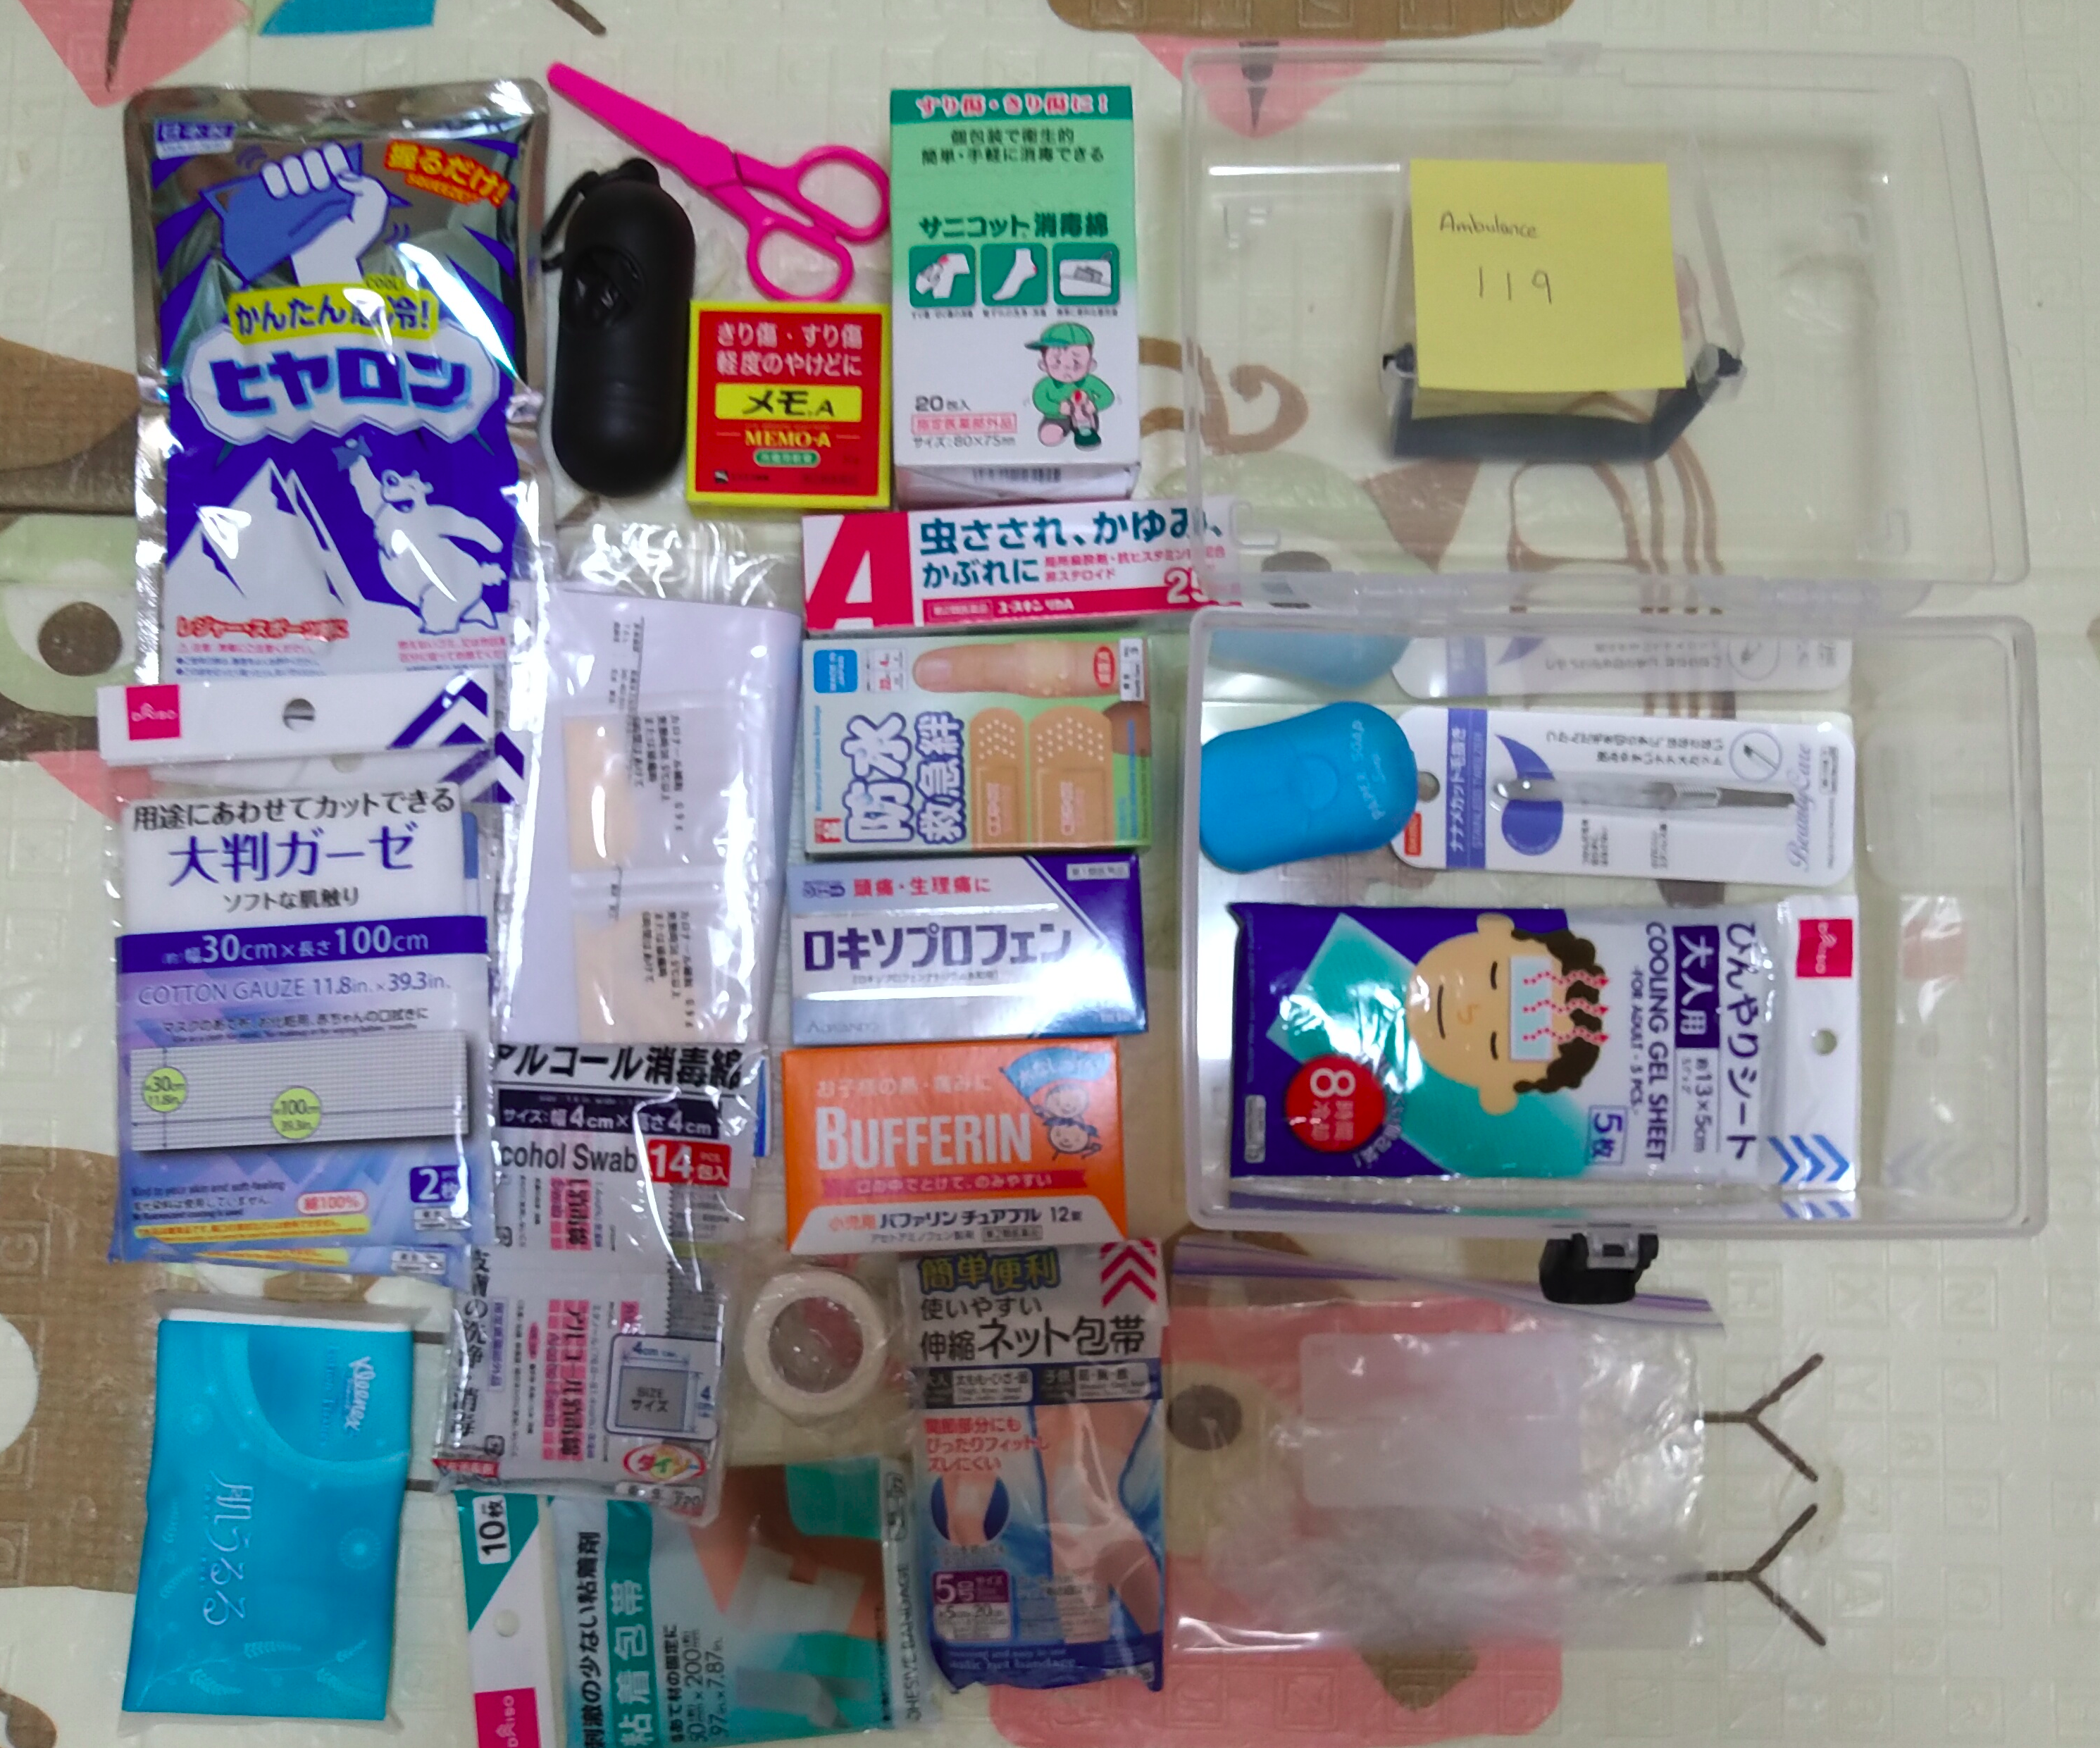
\includegraphics[width=\textwidth, 
height = 0.7\textheight, 
keepaspectratio]
{firstAid}
